\chapter{Исследовательская часть}

В данном разделе будет произведено исследование зависимости качества изображения от доступного набора символов.

Для оценки качества изображения будут исследованы две его составляющие: качество отображения освещенности и качества передачи формы.

\section{Выбор входных параметров}

Сравниваться будут два набора символов:
\begin{enumerate}
    \item полный набор из 128 символов ASCII;
    \item набор из 32 символов ASCII.
\end{enumerate}

Символы для второго набора были выбраны следующим образом:
\begin{enumerate}
    \item сортировка всех символов по яркости (количеству пикселей в их растровом представлении);
    \item добавление каждого четвёртого символа в набор.
\end{enumerate}

Для сравнения были построены изображения следующих объектов:
\begin{enumerate}
    \item сфера с радиусом 5 и центром в начале координат, освещённая источником света (-10, -10, -10);
    \item каркас куба с длиной ребра 2.
\end{enumerate}

Оценка качества отображения освещенности объекта будет производиться по изображениям первого объекта, а оценка качества передачи формы ребер объекта будет производиться по изображениям второго.

Остальные входные данные являются фиксированными.

\section{Проведение исследования}

С выбранными входными данными были построены изображения \ref{fig:brfull}-\ref{fig:shapequat}.

\begin{figure}[H]
    \centering
    \begin{minipage}{0.41\textwidth}
        \centering
        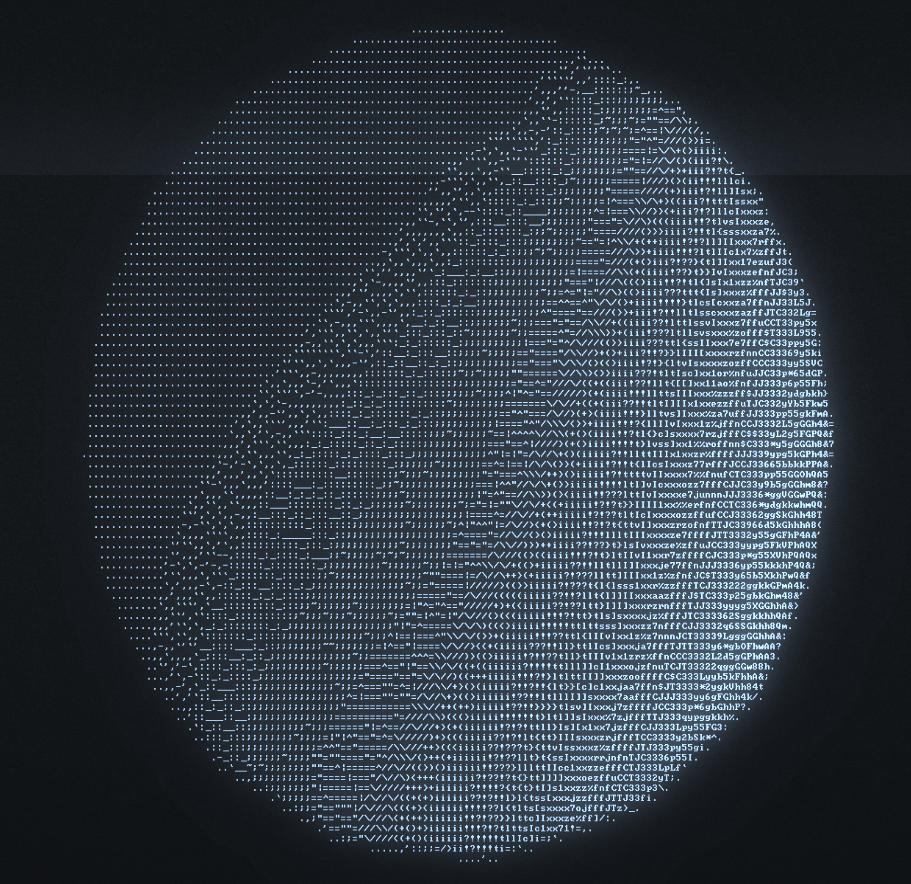
\includegraphics[width=\linewidth]{brfull.png}
        \caption{Набор 1}
	\label{fig:brfull}
    \end{minipage}
    \begin{minipage}{0.36\textwidth}
        \centering
        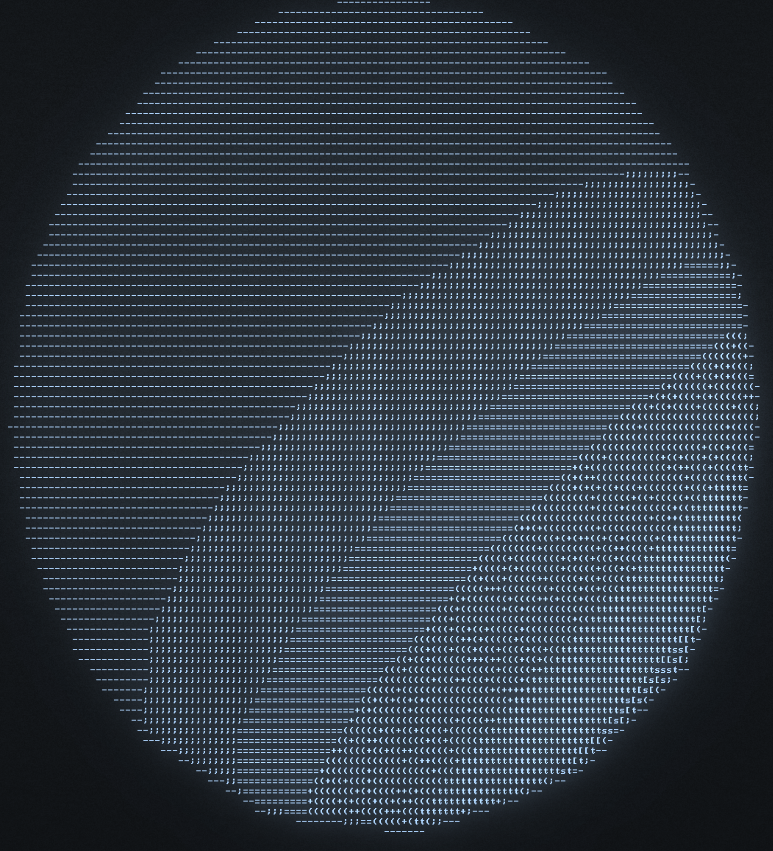
\includegraphics[width=\linewidth]{brquat.png}
        \caption{Набор 2}
	\label{fig:brquat}
    \end{minipage}
\end{figure}

\begin{figure}[H]
    \begin{minipage}{0.43\textwidth}
        \centering
        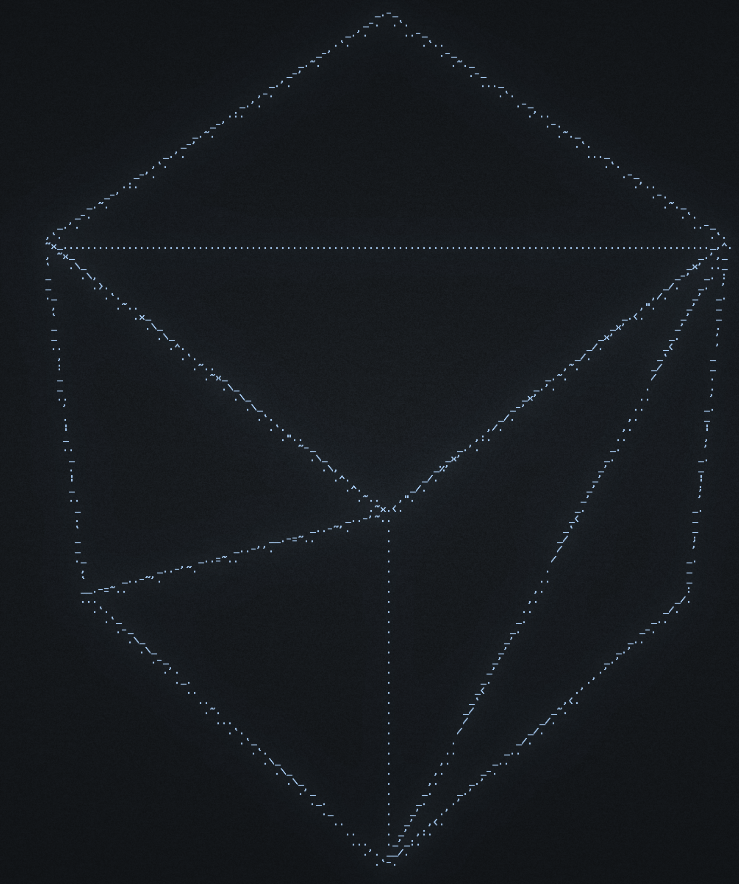
\includegraphics[width=\linewidth]{images/shapefull.png}
        \caption{Набор 1}
	\label{fig:shapefull}
    \end{minipage}
    \begin{minipage}{0.45\textwidth}
        \centering
        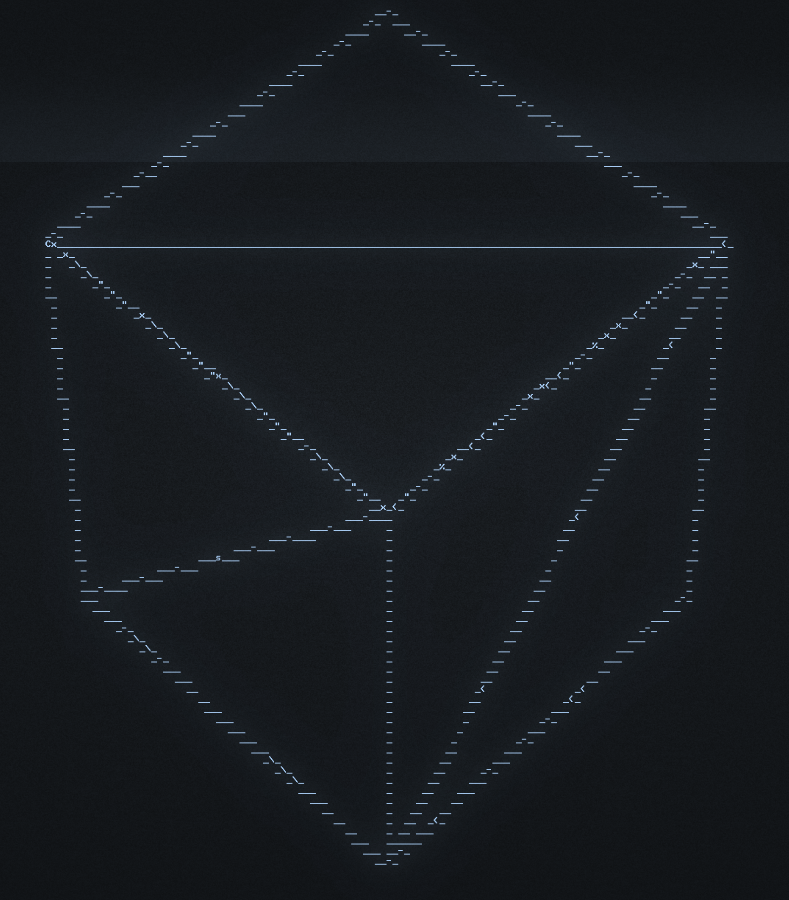
\includegraphics[width=\linewidth]{images/shapequat.png}
        \caption{Набор 2}
	\label{fig:shapequat}
    \end{minipage}
\end{figure}

Данные изображения были помещены в социальный опрос со следующими вопросами:

В отношении первой фигуры, для каждого из наборов:
\begin{enumerate}
    \item Кажется ли вам, что объект на изображении имеет форму сферы?
    \item Вы видите на объекте правдоподобные блики?
    \item Вы ощущаете глубину изображения, как если бы это был трехмерный объект?
    % \item Заметны ли переходы между областями освещенности?
    \item Выберите, где, по вашему мнению, может находиться источник света (справа сверху, справа снизу, слева сверху, слева снизу).
\end{enumerate}

В отношении второй фигуры, для каждого из наборов:
\begin{enumerate}
    \item Кажется ли вам, что объект на изображении имеет форму куба?
    \item Чётко ли вы видите рёбра объекта?
    \item Все ли рёбра объекта выглядят прямыми?
\end{enumerate}

Для проведения опроса использовалась платформа Yandex Forms~\cite{forms}. Данный опрос был пройден 54 людьми. Результаты опроса представлены на рисунках \ref{fig:qna1} и \ref{fig:qna2}.

\begin{figure}[H]
    \centering
    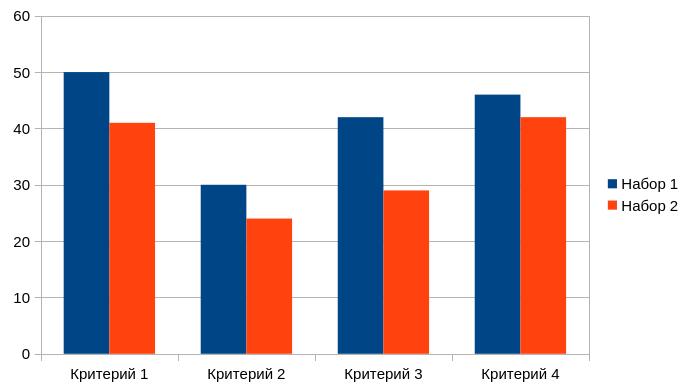
\includegraphics[scale=0.5]{images/qna1.png}
    \caption{Результаты опроса для фигуры 1}
    \label{fig:qna1}
\end{figure}

Из результатов следует, что сокращенный набор символов негативно повлиял на качество отображения освещенности объекта. 

\begin{figure}[H]
    \centering
    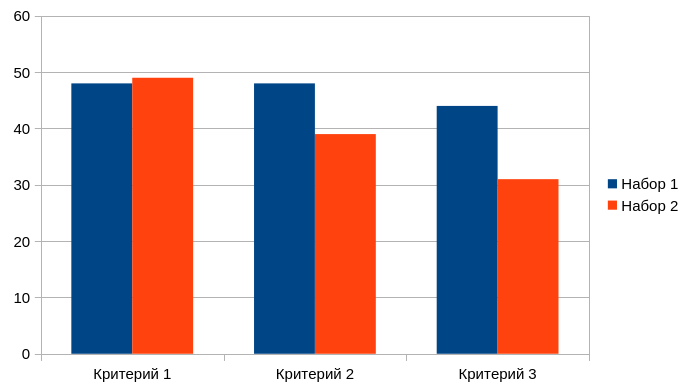
\includegraphics[scale=0.5]{images/qna2.png}
    \caption{Результаты опроса для фигуры 2}
    \label{fig:qna2}
\end{figure}

Из результатов следует, что сокращенный набор символов негативно повлиял на качество отображения формы рёбер объекта.

\section{Выводы из исследовательской части}

В результате проведенного исследования была установлена зависимость качества изображения от используемого набора символов. Сравнение двух наборов символов — полного набора из 128 символов ASCII и сокращенного набора из 32 символов ASCII — показало, что уменьшение количества символов негативно сказывается как на восприятии освещенности, так и на передаче формы объектов.

\clearpage
